\renewcommand{\theequation}{\theenumi}
\begin{enumerate}[label=\arabic*.,ref=\thesubsection.\theenumi]
\numberwithin{equation}{enumi}

\item Express the following equation in the form given in \eqref{eq:quadratic_vec}
\begin{equation}
E:\, 5x_1^2-6x_1x_2 + 5x_2^2+22x_1-26x_2+29=0
\label{eq:ellipse}
\end{equation}
\\
\solution \eqref{eq:ellipse} can be expressed as
\begin{equation}
\vec{x}^TV\vec{x} + 2\vec{u}^T\vec{x}  + 29=0
\label{eq:ellipse_quadc}
\end{equation}
%
where
\begin{equation}
V = \myvec{5 & -3 \\ -3 & 5}, \vec{u} = \myvec{11 \\ -13}
\label{eq:ellipsevu}
\end{equation}
%\item Find $\vec{c}$ and $K$ such that 
%\begin{equation}
%\brak{\vec{x}-\vec{c}}^TV\brak{\vec{x}-\vec{c}} = K 
%\label{eq:ellipsec}
%\end{equation}
%%
%\solution \eqref{eq:ellipsec} can be expressed as
%\begin{align}
%\vec{x}^TV\vec{x}-2\vec{c}^TV\vec{x} +\vec{c}^TV\vec{c}-K = 0.
%\end{align}
%%
%Comparing with \eqref{eq:ellipse_quadc},
%\begin{align}
%V\vec{c}&=-\vec{u}
%\\
%\vec{c}^TV\vec{c} - K &=29
%\\
%\implies \vec{c} &=-V^{-1}\vec{u} = \myvec{-1 \\ 2},
%\\
%\text{and }K& = 8
%\end{align}
%
\item Using the affine transformation in \eqref{eq:affine}, show that 
\eqref{eq:ellipse_quadc} can be expressed as
\begin{equation}
\vec{y}^TD\vec{y}= 1
\label{eq:ellipseo}
\end{equation}
%
where
\begin{align}
\label{eq:ellipse_parmas_d}
\vec{D} &= 
\vec{P}^T\vec{V}\vec{P}
\\
\vec{c}&= -\vec{V}^{-1}\vec{u}
\label{eq:ellipse_parmas_c}
\end{align}
for 
\begin{equation}
\vec{P}^\vec{T}\vec{P} = \vec{I}
\label{eq:ellipse_trans}
\end{equation}
\item Find $\vec{c}$
%For 
\\
\solution 
\begin{align}
%\vec{y}= \frac{P^T\brak{\vec{x}-\vec{c}}}{\sqrt{K}},
\vec{c} = \myvec{1 \\ -2}
%\label{eq:ellipse_xy}
\end{align}
%\eqref{eq:ellipsec} transforms to \eqref{eq:ellipseo}.
\item If 
\begin{align}
D &= \myvec{\lambda_1 & 0 \\ 0 & \lambda_2 }
\\
P &= \myvec{\vec{P}_1 & \vec{P}_2 }
\label{eq:ellipse_eigmat}
\end{align}
show that 
\begin{equation}
V\vec{z} = \lambda \vec{z}
\label{eq:ellipse_eig}
\end{equation}
%
where $\lambda \in \cbrak{\lambda_1, \lambda_2}, \vec{z}\in\cbrak{ \vec{P}_1, \vec{P}_2}$.
\item Find $\lambda$.
\\
\solution $\lambda$ is obtained by solving the following equation.
%\item Find the length of the semi-major and semi-minor axes of $E$.
%\\
%\solution The values are given by
%\begin{align}
%\sqrt{\frac{K}{\lambda}}
%\label{eq:ellipsekl}
%\end{align}
%obtained by solving for $\lambda$ in \eqref{eq:ellipse_eig}.  Thus,
\begin{align}
\abs{\lambda I-V} &= 0
\label{eq:ellipse_ceq}
\\
\implies\begin{vmatrix}\lambda -5 & 3 \\ 3 & \lambda -5\end{vmatrix} & = 0
\\
\implies \lambda^2 -10 \lambda+ 16 &= 0
\\
\implies \lambda &= 2, 8
\end{align}
%Thus, the length of the semi-major axis is 2 and that of the semi-minor axis is 1.
\item Sketch \ref{eq:ellipseo}.
\item Find $\vec{P}_1$ and $\vec{P}_2$.
\\
\solution From \eqref{eq:ellipse_eig}
\begin{align}
V\vec{P}_1 &= \lambda_1 \vec{P}_1
\\
\implies \brak{V-\lambda I} \vec{y}&= 0
\\
\implies \myvec{1 & -1} \vec{P}_1&= 0
\\
\text{or, } \vec{P}_1 = k_1 \myvec{1 \\ 1}
\label{eq:ellipsen1}
\end{align}
%
Similarly, 
%where
%\begin{align}
%\vec{n}_1= \myvec{1 \\ -1}
%\end{align}
%
%Similarly, $\vec{P}_2$ is a point on
\begin{align}
\myvec{1 &  1}\vec{P}_2&= 0
\\
\text{or, } \vec{P}_2 = k_2 \myvec{1 \\ -1}
\end{align}
%
%\begin{align}
%\vec{n}_2= 
%\end{align}
\item Find $\vec{P}$.
\\
\solution From \eqref{eq:ellipse_trans} and \eqref{eq:ellipse_eigmat},
\begin{align}
k_1 &=  \frac{1}{\norm{\myvec{1 \\ 1}}} = \frac{1}{\sqrt{2}}
\\
k_2 &=  \frac{1}{\norm{\myvec{1 \\ -1}}} = \frac{1}{\sqrt{2}}
\end{align}
%
Thus,
\begin{align}
\vec{P} = \frac{1}{\sqrt{2}}\myvec{1 & 1 \\ 1 & -1}
\end{align}

\item Find the equation of the major axis for $E$.
\\
\solution  The major axis for \eqref{eq:ellipseo} is the line
\begin{equation}
\vec{y} = \lambda_1\myvec{1 \\ 0}.
\end{equation}
Using the affine transformation in \eqref{eq:affine}
\begin{align}
\vec{x}= \vec{P}\vec{y}+\vec{c}
\\ 
\implies  \vec{x}-\vec{c}= \lambda_1\vec{P}_1
\\ 
\text{or, }\myvec{1 & -1}\vec{x}&= \myvec{1 & -1}\myvec{1 \\ -2}
\\
&= -3
\end{align}
%
since 
\begin{align}
P\myvec{1 \\ 0}=\vec{P}_1\text{ and } \myvec{1 & -1}\vec{P}_1 = 0
\end{align}
%
which is the major axis of the ellipse $E$.
\item Find the minor axis of $E$.
%
\item Let $\vec{F}_1,\vec{F}_2$ be such that
\begin{equation}
\norm{\vec{x}-\vec{F}_1}
+\norm{\vec{x}-\vec{F}_2} =2k
\end{equation}
Find $\vec{F}_1, \vec{F}_2$ and $k$.
\item 
%Summarize all the above computations through a Python script and 
Plot 
the ellipses in \eqref{eq:ellipse} and \eqref{eq:ellipseo}.
\\
\solution 
%The following script plots 
See Fig. \ref{fig:ellipse} 
%using the 
%principles of an affine transformation. 
%\begin{lstlisting}
%https://github.com/gadepall/school/raw/master/linalg/2D/manual/codes/ellipse.py
%\end{lstlisting}
\begin{figure}[!ht]
\centering
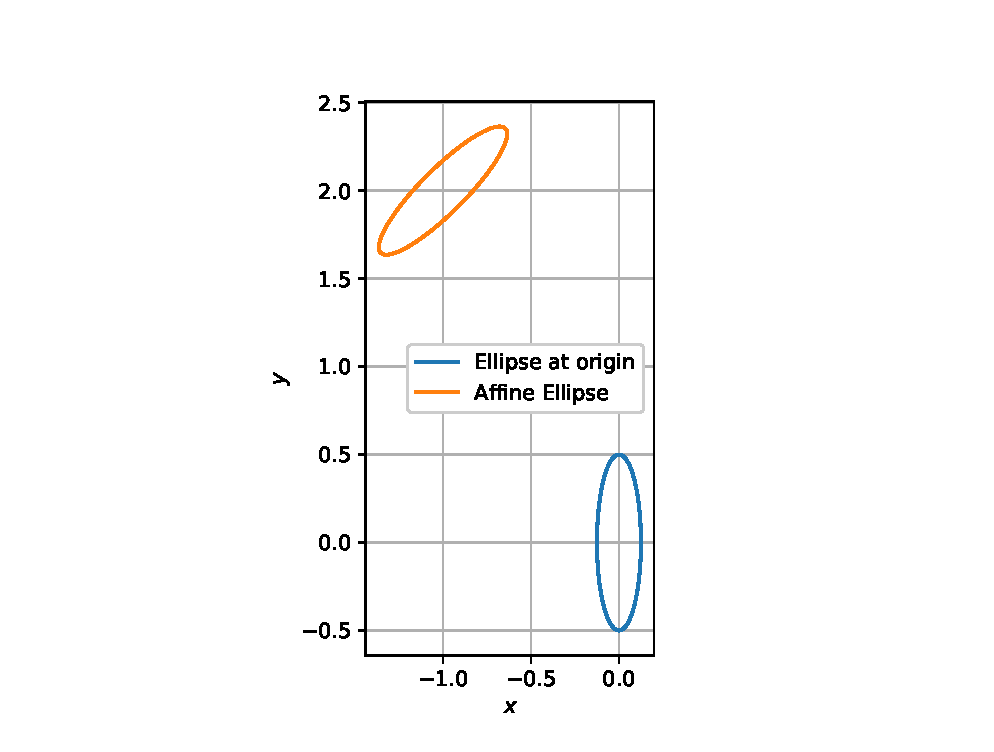
\includegraphics[width=\columnwidth]{./figs/ellipse.eps}
\caption{}
\label{fig:ellipse}
\end{figure}
\end{enumerate}
